\documentclass[11pt]{amsart}
\usepackage{hyperref}
\usepackage{geometry}                % See geometry.pdf to learn the layout options. There are lots.
\geometry{letterpaper}                   % ... or a4paper or a5paper or ... 
%\geometry{landscape}                % Activate for for rotated page geometry
\usepackage[parfill]{parskip}    % Activate to begin paragraphs with an empty line rather than an indent
\usepackage{graphicx}
\usepackage{amssymb}
\usepackage[all]{xy}
\usepackage{epstopdf}
\usepackage{color}
\usepackage[cache=false]{minted}
\DeclareGraphicsRule{.tif}{png}{.png}{`convert #1 `dirname #1`/`basename #1 .tif`.png}


% these packages make it easy to include figures in the text. 
\usepackage{float}
\restylefloat{figure}
% newcommand
\newcommand{\ip}[1]{\left\langle #1\right\rangle}



\begin{document}
{\Large Name: Philip Pham}  \\
\begin{center}
\Large AMATH 515 \hskip 2in Homework Set 3\\
{\bf Due: Monday, March 9th by midnight.}. 
\end{center}
\bigskip
\begin{enumerate}

\item  Compute the conjugates of the following functions.  
\begin{enumerate}
\item $f(x) = \delta_{\mathbb{B}_{\infty}}(x)$.
  \begin{proof}
    We have that
    \begin{equation*}
      \boxed{
        f^\star(x) =
        \delta^\star_{\mathbb{B}_{\infty}}(x)
        = \max_{y \in \mathbb{B}_{\infty}} \left\langle x, y \right\rangle
        = \sum_i \left|x_i\right|.}
    \end{equation*}

    By definition,
    \begin{equation*}
      f^\star(x) = \sup_{y}\left\{\left\langle x, y \right\rangle - f(y)\right\}.           
    \end{equation*}
    If $y \not\in \mathbb{B}_{\infty}$, then
    $\left\langle x, y \right\rangle - f(y) = -\infty$ for all $x$. For
    $y \in \mathbb{B}_{\infty}$,
    $\left\langle x, y \right\rangle - f(y) = \left\langle x, y \right\rangle$,
    so to maximize $\left\langle x, y \right\rangle - f(y)$, we should choose
    $y$ such that $\left\langle x, y \right\rangle$ is maximized.
  \end{proof}
\item $f(x) = \delta_{\mathbb{B}_{2}}(x)$.
  \begin{proof}
    We have that
    \begin{equation*}
      \boxed{
        f^\star(x) =
        \delta^\star_{\mathbb{B}_{2}}(x)
        = \max_{y \in \mathbb{B}_{2}} \left\langle x, y \right\rangle
        = \left\|x\right\|_2.}      
    \end{equation*}
    
    The proof is identical to the previous one with $\mathbb{B}_{\infty}$
    replaced by $\mathbb{B}_2$.
  \end{proof}
\item $f(x) = \exp(x)$.
  \begin{proof}
    We have that
    \begin{equation*}
      \boxed{f^\star(x) =
        \begin{cases}
          x\log x - x = x\left(\log x - 1\right), &x > 0; \\
          0, &x = 0; \\
          \infty, &x < 0.
        \end{cases}}
    \end{equation*}

    To see this, we can maximize
    $\left\langle x, y \right\rangle - \exp\left(y\right)$ with respect to $y$
    by taking the derivative, setting it to $0$, and solving for $y$. In doing
    so, we find that $y = \log x$, which is only defined when $x > 0$. When
    $x \leq 0$, we see that we can maximize $xy - \exp\left(y\right)$ by sending
    $y$ to $-\infty$.
  \end{proof}
\item $f(x) =  \log(1+\exp(x))$
  \begin{proof}
    We have that
    \begin{equation*}
      \boxed{f^\star(x) =
        \begin{cases}
          \infty, &x > 1; \\
          0, &x = 1; \\
          x\log x + \left(1 - x\right)\log\left(1 - x\right), & 0 < x < 1; \\
          0, & x = 0; \\
          \infty, &x < 0.
        \end{cases}}
    \end{equation*}

    Consider $xy - \log(1+\exp(y))$. The derivative with respect to $y$ is
    $x - \frac{\exp(y)}{1+\exp(y)}$. When $x \in \left(0, 1\right)$, we can
    solve for $y = \log\left(\frac{x}{1 - x}\right)$. When $x \geq 1$, the
    derivative is always positive, so we have that the max is obtained when
    $y \rightarrow \infty$. We note that
    \begin{equation*}
      xy - \log(1+\exp(y)) = xy - \left[
        y + \exp(-y) - \frac{\exp(-2y)}{2} + \frac{\exp(-3y)}{3} - \frac{\exp(-4y)}{4} + \cdots
      \right]
    \end{equation*}
    by a Taylor series expansion, so as $y \rightarrow \infty$, we have $\infty$
    if $x > 1$ and $0$ if $x = 1$.

    When $x \leq 0$, the derivative is always negative, so we maximize the
    expression with $y \rightarrow -\infty$. When $x = 0$, only the second term
    remains, so we have $0$. If $x < 0$, we have that the first term tends to
    $\infty$ and the second term tends to $0$.
  \end{proof}
\item $f(x) = x\log(x)$
  \begin{proof}
    We have that
    \begin{equation*}
      \boxed{f^\star(x) = \exp\left(x - 1\right).}
    \end{equation*}

    We can take the derivative of $xy - y\log y$ with respect to $y$, set this
    equal to $0$, and solve for $y$. We find that $y = \exp\left(x -
      1\right)$. Substituting, we obtained the desired result.
  \end{proof}
\end{enumerate}


\bigskip\bigskip



\item  Let $g$ be any convex function; $f$ is formed using $g$.
Compute $f^\star$ in terms of $g^\star$.  
\begin{enumerate}
\item $f(x) = \lambda g(x)$.
  \begin{proof}
    \begin{equation*}
      \boxed{f^\star\left(x\right)
      = \lambda g^\star\left(\frac{x}{\lambda}\right)}
    \end{equation*}

    To see this,
    \begin{align*}
      f^\star\left(x\right)
      &= \sup_{y} \left\{\left\langle x, y \right\rangle - f(y)\right\} \\
      &= \sup_{y} \left\{\left\langle x, y \right\rangle - \lambda g(y)\right\} \\
      &= \lambda \sup_{y}
        \left\{\left\langle \frac{x}{\lambda}, y \right\rangle - g(y)\right\} \\
      &= \lambda g^\star\left(\frac{x}{\lambda}\right).
    \end{align*}
  \end{proof}
\item $f(x) = g(x-a) + \langle x, b \rangle$.
  \begin{proof}
    \begin{equation*}
      \boxed{f^\star\left(x\right)
        = \left\langle x - b, a \right\rangle + g^\star\left(x - b\right)}
    \end{equation*}
    
    \begin{align*}
      f^\star\left(x\right)
      &= \sup_{y} \left\{\left\langle x, y \right\rangle - f(y)\right\} \\
      &= \sup_{y} \left\{\left\langle x, y \right\rangle - g(y - a)\right\} \\
      &= \sup_{y} \left\{\left\langle x, y \right\rangle -
        \left\langle y, b \right\rangle - g(y - a)\right\} \\
      &= \sup_{y} \left\{\left\langle x - b, y \right\rangle - g(y - a)\right\} \\
      &= \sup_{y} \left\{
        \left\langle x - b, a \right\rangle + 
        \left\langle x - b, y - a \right\rangle - g(y - a)\right\} \\
      &= \left\langle x - b, a \right\rangle + \sup_{y} \left\{
        \left\langle x - b, y - a \right\rangle - g(y - a)\right\} \\
      &= \left\langle x - b, a \right\rangle + g^\star(x - b)
    \end{align*}
    since shiftfing by $a$ does not change the supremum.
  \end{proof}
\item $f(x) = \inf_z \left\{g(x,z)\right\}$.
  \begin{proof}
    Rewrite $g(x,z) = g_z(x)$ to emphasize that we're conjugating on the $x$
    argument. Then, we have that
    \begin{equation*}
      \boxed{f^\star\left(x\right) = \sup_z g_z^\star(x).}
    \end{equation*}

    Since
    \begin{equation*}
      \sup_{y} \left\{\left\langle x, y \right\rangle - \inf_zg(y, z)\right\}
      \geq
      \sup_{y} \left\{\left\langle x, y \right\rangle - g(y, z)\right\}
    \end{equation*}
    for all $z$, and we can choose $z$ so that the right-hand size is
    arbitrarily close to the left-hand size, we have that
    \begin{equation*}
      f^\star\left(x\right)
      = \sup_{y} \left\{\left\langle x, y \right\rangle - \inf_zg(y, z)\right\}
      = \sup_z\sup_{y} \left\{\left\langle x, y \right\rangle - g(y, z)\right\}.
    \end{equation*}

    Since
    $g^\star_z(x) = \sup_{y} \left\{\left\langle x, y \right\rangle - g(y,
      z)\right\}$, we have our desired result.        
  \end{proof}
\item $f(x) = \inf_z \left\{\frac{1}{2}\|x-z\|^2 + g(z)\right\}$
  \begin{proof}
    Let $h_z(x) = \frac{1}{2}\|x-z\|^2 + g(z)$.


    Noting that the conjugate of $\|x\|^2/2$ is itself, we can apply part (b) to
    obtain
    $h_z^\star(x) = \frac{1}{2}\|x\|^2 + \left\langle x, z\right\rangle - g(z)$.

    Applying the results of part (c), we have that
    \begin{equation*}
      f^\star\left(x\right)
      = \sup_z \left\{\frac{1}{2}\|x\|^2 + \left\langle x, z\right\rangle - g(z)\right\}
      = \boxed{\frac{1}{2}\|x\|^2 + g^\star(x).}
    \end{equation*}    
  \end{proof}
\end{enumerate}

\bigskip\bigskip

\item Moreau Identities.
\begin{enumerate}
\item  Derive the Moreau Identity: 
\[
\mbox{prox}_{f}(z) + \mbox{prox}_{f^\star}(z) = z. 
\]

\begin{proof}
  It follows from Corollary 4.41 of the text:
  \begin{equation*}
    y \in \partial f (x) \Leftrightarrow x \in \partial f^\star(y).
  \end{equation*}

  We also use Proposition 4.39 to note that
  \begin{align*}
    \operatorname{prox}_{f}(z) = \arg\min_x f(x) + \frac{1}{2}\left\|x - z\right\|^2
    &\Leftrightarrow 0 \in \partial \left(
      f\left(\operatorname{prox}_{f}(z)\right) + \frac{1}{2}\left\|\operatorname{prox}_{f}(z) - z\right\|^2\right) \\
    &\Leftrightarrow
      z - \operatorname{prox}_{f}(z) \in \partial f\left(\operatorname{prox}_{f}(z)\right).
  \end{align*}
  
  So we use these two facts to find that
  \begin{align*}
    z - \mbox {prox}_{f}(z) \in \partial f \left(\mbox{prox}_{f}(z)\right)
    &\Leftrightarrow \mbox{prox}_{f}(z) \in \partial f^\star
      \left(z - \mbox {prox}_{f}(z)\right)\\
    &\Leftrightarrow
      z - \left(z - \mbox{prox}_{f}(z)\right) \in \partial f^\star
      \left(z - \mbox{prox}_{f}(z)\right) \\
    &\Leftrightarrow
      \mbox{prox}_{f^\star}(z) = z - \mbox{prox}_{f}(z) \\
    &\Leftrightarrow z = \mbox{prox}_{f}(z) + \mbox{prox}_{f^\star}(z),
  \end{align*}
  which is our desired result.
  
\end{proof}
%\item Take a look at this more detailed identity:  
%\[
%\mbox{prox}_{\alpha f}(z) = z - \alpha \mbox{prox}_{\frac{1}{\alpha}f^*}(z/\alpha).
%\]
%Don't prove this, but please remember it --- its very useful for coding. 


\item Use either of the Moreau identities and 1a, 1b to check your formulas for
\[
\mbox{prox}_{\|\cdot\|_1}, \quad \mbox{prox}_{\|\cdot\|_2}
\]
from last week's homework.

\begin{proof}
  For $\mbox{prox}_{\|\cdot\|_1}$, we note that
  \begin{align*}
    \left(\|x\|_1\right)^\star
    &= \sup_y \left\{\left\langle x, y \right\rangle - |y|_1\right\} \\
    &= \sup_y \left\{\sum_i x_iy_i - |y_i|\right\} \\
    &= \begin{cases}
      \infty, &\text{if any $\left|x_i\right| > 1$}; \\
      0, &\text{otherwise.}
    \end{cases}
  \end{align*}

  Thus, the proximal operator is
  \begin{align*}
    \mbox{prox}_{\left(\|\cdot\|_1\right)^\star}\left(x\right)
    &= \arg\min_y\frac{1}{2}\left\|y - x\right\|^2 + \left(\|y\|_1\right)^\star \\
    &= \min(\left|x\right|, 1)\operatorname{sign}\left(x\right),
  \end{align*}
  where I have abused notation and all operations are done element-wise.
  

  Then, applying the Moreau identity, we obtain
  \begin{align*}
    \mbox{prox}_{\|\cdot\|_1} (x)
    &= x - \mbox{prox}_{\left(\|\cdot\|_1\right)^\star} (x) \\
    &= x - \min(\left|x\right|, 1)\operatorname{sign}\left(x\right) \\
    &= \operatorname{sign}\left(x\right)\max\left(\left|x\right| - 1, 0\right),
  \end{align*}
  which agrees with my previous result.
  
  We have that
  \begin{align*}
    \left(\|x\|_2\right)^\star
    &= \sup_y \left\{\left\langle x, y\right\rangle - \|\ y \|_2\right\} \\
    &\geq \|\ x \|_2 \|\ y \|_2 - \|\ y \|_2 \\
    &\geq \|\ y \|_2\left(\|\ x \|_2  - 1\right),
  \end{align*}
  where we have equality if we choose $y$ in the same direction as $x$. Thus,
  we'll have that $\left(\|x\|_2\right)^* = \infty$ if $\|\ x \|_2 > 1$ and
  $\left(\|x\|_2\right)^* = 0$ if $\|\ x \|_2 \leq 1$.

  Then, we have that
  \begin{align*}
    \mbox{prox}_{\left(\|\cdot\|_2\right)^\star} (x)
    &= \arg\min_y\frac{1}{2}\left\|y - x\right\|^2 + \left(\|y\|_2\right)^\star \\
    &= \begin{cases}
      x, &\|x\|_2 \leq 1; \\
      \frac{x}{\|x\|_2}, &\|x\|_2 > 1.
    \end{cases}
  \end{align*}
  
  Then, applying the Moreau identity, we obtain
  \begin{align*}
    \mbox{prox}_{\|\cdot\|_2} (x)
    &= x - \mbox{prox}_{\left(\|\cdot\|_2\right)^\star} (x) \\
    &= \begin{cases}
      0, &\|x\|_2 \leq 1; \\
      x\left(1 - \frac{1}{\|x\|_2}\right), &\|x\|_2 > 1.
    \end{cases}
  \end{align*}
  This agrees with my previous result for $\mbox{prox}_{\|\cdot\|_2}$.
  
\end{proof}
\end{enumerate}



%\item Consider the following linear program: 
%\[
%\min_x c^Tx \quad \mbox{s.t.} \quad Ax \leq b, \quad x \geq 0.
%\] 
%Derive the dual problem we get from the perturbation 
%\[
%p(u) = \min_{x} c^Tx \quad \mbox{s.t.} \quad Ax \leq b + u, \quad x \geq 0.
%\]

%\bigskip\bigskip\bigskip

%\item{Duals of Lasso Formulations}
%
%\begin{enumerate}
%
%\item Compute the dual of  the constrained Lasso problem
%\[
%\min_{x} \frac{1}{2}\|b - Ax\|^2 \quad \mbox {s.t.} \quad \|x\|_1 \leq \tau. 
%\]
%obtained from the perturbation 
%\[
%p(u) = \min_{x} \frac{1}{2}\|b - Ax + u\|^2 \quad \mbox {s.t.} \quad \|x\|_1 \leq \tau. 
%\]
%
%\bigskip\bigskip
%
%\item Compute the dual for the modified problem  
%\[
%\min_{x} \|b - Ax\|_2 +\lambda \|x\|_1. 
%\]
%obtained from perturbation 
%\[
%p(u) = \min_{x} \|b - Ax + u\|_2 +\lambda \|x\|_1. 
%\]
%
%
%\end{enumerate}
%
%\bigskip\bigskip\bigskip

\item Duals of regularized GLM. Consider the Generalized Linear Model family: 
\[
\min_{x} \sum_{i=1}^n g(\langle a_i, x\rangle) - b^TAx + R(x),
\]
Where $g$ is convex and $R$ is any regularizer. 
\begin{enumerate}
\item Write down the general dual obtained from the perturbation 
\[
p(u) = \min_{x} \sum_{i=1}^n g(\langle a_i, x\rangle + u_i) - b^TAx + R(x).
\]

\begin{proof}
  Let
  \begin{equation*}    
    f_x\left(u\right) = \sum_{i=1}^n g(\langle a_i, x\rangle + u_i) - b^TAx + R(x).
  \end{equation*}

  By Problem (2)(c),
  \begin{align*}        
    p^\star\left(u\right)
    &= \sup_x\left\{f_x^\star\left(u\right)\right\}.
  \end{align*}

  By Problem (2)(b),
  \begin{align*}
    f_x^\star\left(v\right)
    &= \sup_u\left\{
      \left\langle v, u\right\rangle
      - \left[\sum_{i=1}^n g(\langle a_i, x\rangle + u_i) - b^TAx + R(x)\right]\right\} \\
    &= \sup_u\left\{
      \sum_{i=1}^n \left[v_iu_i - g(\langle a_i, x\rangle + u_i)\right] +
      \left[b^TAx - R(x)\right]
      \right\} \\
    &= b^TAx - R(x) + \sup_u\left\{
      \sum_{i=1}^n \left[v_iu_i - g(\langle a_i, x\rangle + u_i)\right]\right\} \\
    &= b^TAx - R(x) + 
      \sum_{i=1}^n \sup_{u_i}\left\{v_iu_i - g(\langle a_i, x\rangle + u_i)\right\} \\
    &=  b^TAx - R(x) + \sum_{i=1}^n\left[
      g^\star\left(v_i\right) -v_i\langle a_i, x\rangle \right] \\
    &=  b^TAx - R(x) - v^TAx
      + \sum_{i=1}^ng^\star\left(v_i\right).
  \end{align*}

  Thus, we have that
  \begin{align*}
    p^\star\left(u\right)
    &= \sup_x \left\{b^TAx - R(x) - u^TAx + \sum_{i=1}^ng^\star\left(u_i\right)\right\} \\
    &= \sum_{i=1}^ng^\star\left(u_i\right) + \sup_x \left\{\left(b - u\right)^TAx - R(x)\right\} \\
    &= \sum_{i=1}^ng^\star\left(u_i\right) + R^\star\left(A^T\left(b - u\right)\right).
  \end{align*}
\end{proof}

\item Specify your formula to Ridge-regularized logistic regression: 
\[
\min_x \sum_{i=1}^n \log(1+\exp(\langle a_i, x \rangle))  - b^TAx  + \frac{\lambda}{2}\|x\|^2. 
\]

\begin{proof}
  Using the results in from Problem (1)(d) and Problem (2)(a), we have that
  \begin{align*}
    g(x) = \log(1 + \exp\left(x\right))
    &\Rightarrow
      g^\star(x) = \begin{cases}
        \infty, &|2x - 1| > 1; \\
        0, &|2x - 1| = 1; \\
        x\log x + \left(1 - x\right) \log\left(1 - x\right), &\text{otherwise};
      \end{cases}
    \\
    R(x) = \frac{\lambda}{2}\|x\|^2
    &\Rightarrow R^\star(x) = \frac{1}{2\lambda}\|x\|^2 \\
  \end{align*}

  We can substitute to get
  \begin{equation*}
    p(u) = \sum_{i=1}^ng^\star\left(u_i\right) + \frac{1}{2\lambda}\|A^T\left(b - u\right)\|^2.
  \end{equation*}
\end{proof}

\item Specify your formula to 1-norm regularized Poisson regression: 
\[
\min_x \sum_{i=1}^n \exp(\langle a_i, x \rangle) - b^TAx +  \lambda\|x\|_1. 
\]
\begin{proof}
  Using the results in from Problem (1)(c), Problem (2)(a), and Problem (3)(b), we have that
  \begin{align*}
    g(x) = \exp(x)
    &\Rightarrow
      g^\star(x) = \begin{cases}
        \infty, &x < 0; \\
        0, &x = 0; \\
        x\left(\log x - 1\right), &\text{otherwise};
      \end{cases}
    \\
    R(x) = \lambda\|x\|_1 &\Rightarrow R^\star(x) = \begin{cases}
      \infty, &\text{if any $\left|x_i\right| > \lambda$}; \\
      0, &\text{otherwise.}
    \end{cases}
  \end{align*}

  We can substitute to get
  \begin{equation*}
    p(u) = \sum_{i=1}^ng^\star\left(u_i\right) + R^\star\left(A^T\left(b - u\right)\right).
  \end{equation*}
\end{proof}


\end{enumerate}
\bigskip \bigskip
\end{enumerate}
\noindent{\bf Coding Assignment}
\vskip 8pt
Please download \texttt{515Hw3\_Coding.ipynb} and \texttt{proxes.py} to complete problem (5).

\vskip 16pt
\begin{enumerate}
\item[(5)] In this problem you will write a routine to project onto the capped simplex. 

The Capped Simplex $\Delta_k$ is defined as follows: 
\[
\Delta_k := \left\{x: \mathbf{1}^Tx = k, \quad 0 \leq x_i \leq 1 \quad \forall i. \right\}
\]
This is the intersection of the $k$-simplex with the unit box. 

The projection problem is given by 
\[
\mbox{proj}_{\Delta_k}(z) = \arg\min_{x \in \Delta_k} \frac{1}{2}\|x-z\|^2.
\]
\begin{enumerate}
\item Derive the (1-dimensional) dual problem by focusing on the $\mathbf{1}^Tx = k$ constraint. 
  \begin{proof}
    We can rewrite the the problem as
    \begin{align*}
      \mbox{proj}_{\Delta_k}(z)
      &= \arg\min_{x \in \Delta_k} \frac{1}{2}\|x-z\|^2 \\
      &= \arg\min_{x \in \mathbb{R}^n} \frac{1}{2}\|x-z\|^2 + \delta_{\{0\}}\left(\mathbf{1}^Tx - k \right) +
        \delta_{[0,1]^n}\left(x \right) \\
      &= \arg\min_{x \in \mathbb{R}^n} \frac{1}{2}\|x-z\|^2 +
        \sup_{\lambda \in \mathbb{R}}\left\{\lambda\left(\mathbf{1}^Tx - k \right)\right\} +
        \delta_{[0,1]^n}\left(x \right) \\
      &= \arg\min_{x \in \mathbb{R}^n} \sup_{\lambda \in \mathbb{R}}\left\{
        \frac{1}{2}\|x-z\|^2 +
        \lambda\left(\mathbf{1}^Tx - k \right) +
        \delta_{[0,1]^n}\left(x \right)
        \right\}.
    \end{align*}

    If $k \in \left(0, n\right]$, we can apply Slater's condition since there is
    guaranteed to be an $x$ such that $x \in [0, 1]^n$ and $\mathbf{1}^Tx =
    k$. Thus, we have strong duality, and
    \begin{align*}
      \min_{x \in \mathbb{R}^n} \sup_{\lambda \in \mathbb{R}}\left\{
        \frac{1}{2}\|x-z\|^2 +
        \lambda\left(\mathbf{1}^Tx - k \right) +
        \delta_{[0,1]^n}\left(x \right)
      \right\} = \\
      \boxed{\sup_{\lambda \in \mathbb{R}}\min_{x \in \mathbb{R}^n}
                \frac{1}{2}\|x-z\|^2 +
        \lambda\left(\mathbf{1}^Tx - k \right) +
      \delta_{[0,1]^n}\left(x\right).}
    \end{align*}        
  \end{proof}
\item Implement a routine to solve this dual. It's a scalar root finding problem, 
  so you can use the root-finding algorithm provided in the code.

  \begin{proof}
    Suppose we fix $\lambda$. The inner minimization problem is solved by
    $\mbox{prox}_{g + h}(z)$, where $g(x) = \lambda\mathbf{1}^Tx - \lambda k$
    and $h\left(x\right) = \delta_{[0,1]^n}\left(x\right)$. Since $g$ is affine,
    we can apply Theorem 3 of Yu's
    \href{http://papers.neurips.cc/paper/4863-on-decomposing-the-proximal-map}{\emph{On
        Decomposing the Proximal Map}} to obtain
    \begin{align*}
      \mbox{prox}_{g + h}(z)
      &= \mbox{prox}_{h}\left(\mbox{prox}_{g}(z)\right) \\
      &= \mbox{prox}_{h}\left(x - \lambda\mathbf{1}\right) \\
      &= \min\left(\left(x - \lambda\mathbf{1}\right)_+, \mathbf{1}\right),
    \end{align*}
    where $\left(\cdot\right)_+ = \max\left(\cdot, 0\right)$, and the $\min$ and
    $\left(\cdot\right)_+$ operation are taken to be element-wise.

    Denote
    $x_\lambda = \min\left(\left(x - \lambda\mathbf{1}\right)_+,
      \mathbf{1}\right)$. With this notation, we have that
    \begin{align*}
      \sup_{\lambda \in \mathbb{R}}\min_{x \in \mathbb{R}^n}
      \frac{1}{2}\|x-z\|^2 +
      \lambda\left(\mathbf{1}^Tx - k \right) +
      \delta_{[0,1]^n}\left(x\right)
      &= \sup_{\lambda \in \mathbb{R}}
        \frac{1}{2}\|x_\lambda-z\|^2 +
        \lambda\left(\mathbf{1}^Tx_\lambda - k \right),
    \end{align*}
    where the last term falls away since $x_\lambda$ is always in the unit
    box. By duality, the solution must occur when
    $\mathbf{1}^Tx_\lambda - k = 0$, so we need to solve for $\lambda$ such that
    \begin{equation*}
      \mathbf{1}^T\min\left(\left(z - \lambda\mathbf{1}\right)_+, \mathbf{1}\right) - k = 0.
    \end{equation*}
    The first term is monotonically decreasing as a function of $\lambda$, so we
    can use bisection to solve for $\lambda$. See \texttt{prox\_csimplex} in
    Listing \ref{lst:prox_csimplex} for a Python implementation.
    
    \begin{listing}
      \small
      \inputminted{python}{proxes.py}
      \caption{An implementation of Equation \ref{eqn:prox_csimplex} in the \texttt{proxes.py} file.}
      \label{lst:prox_csimplex}
    \end{listing}
  \end{proof}
  
\item Using the dual solution, write down a closed form formula for the projection.  
Use this formula, along with your dual solver, to implement the projection. You can use the unit test 
provided to check if your code is working correctly.

\begin{proof}
  \begin{align}
    \mbox{proj}_{\Delta_k}(z)
    &= \min\left(\left(z - \lambda\mathbf{1}\right)_+, \mathbf{1}\right),
      \label{eqn:prox_csimplex} \\
    \text{where $\lambda$ satisfies}~
    0 &= \mathbf{1}^T\min\left(\left(z - \lambda\mathbf{1}\right)_+, \mathbf{1}\right) - k,
    \nonumber
  \end{align}
  where the $\min$ and $\left(\cdot\right)_+$ operation are taken to be
  element-wise.
  
  See Figure \ref{fig:prox_csimplex} for an example of this algorithm.
  \begin{figure}
    \centering
    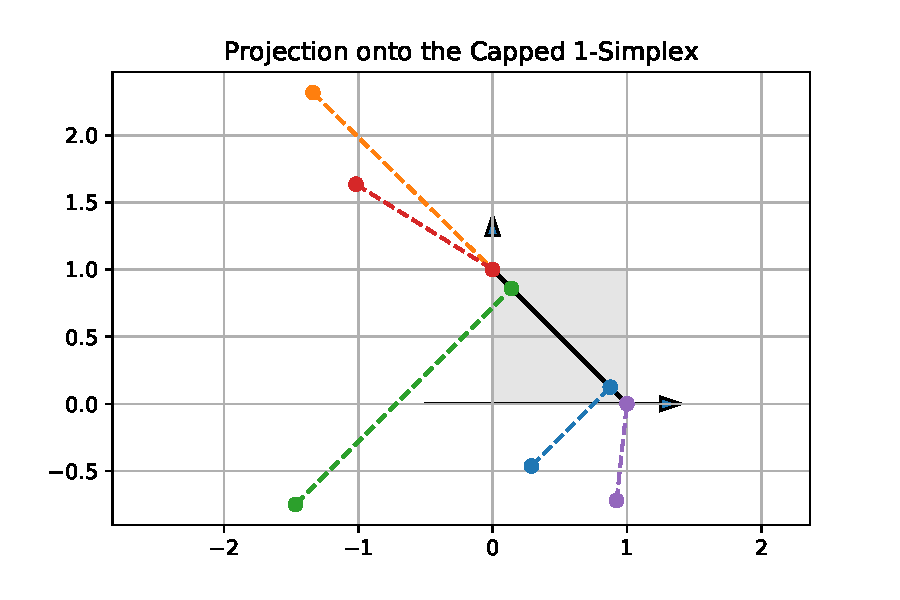
\includegraphics{prox_csimplex.pdf}
    \caption{Projection of 5 randomly-generated points using Equation \ref{eqn:prox_csimplex}.}
    \label{fig:prox_csimplex}
  \end{figure}
\end{proof}

\end{enumerate}

\end{enumerate}

\end{document}
%%% Local Variables:
%%% TeX-command-extra-options: "-shell-escape"
%%% End: